\chapter*{Iconix}
\label{ap1:iconix}

Neste Apêndice serão apresentados os artefatos gerados ao longo do processo de desenvolvimento deste trabalho.

\section*{Fluxos de eventos}

Após a criação do diagrama de casos de uso, foram gerados os fluxos de eventos para cada caso de uso, como serão apresentados a seguir. O primeiro fluxo de eventos gerado é referente ao caso de uso ''Aceitar parceria'', conforme apresenta o Quadro~\ref{ap1:quad:fluxo_evento_aceitar_parceria}.

\captionsetup[quadro]{list=no}
\begin{quadro}[h!]
	\begin{fluxoDeEventos}
  \addTitle{Aceitar Parceria}
  \addrow{Ator principal}{Contratante ou Ambos}
  \addrow{Ator secundário}{-}
  \addrow{Pré-condições}{O ator estar autenticado no sistema}
  \addrow{Pós-condições}{Novo(a) parceiro(a) adicionado(a) a lista de  parceiros do ator.}
  
  \startBasicFlow{Ator} {Sistema}
  \addItemByColumnOne{O ator acessa a página inicial do sistema personalizada a ele.}
  \addItemByColumnTwo{O sistema busca em sua base de dados todas as requisições de parcerias pendentes ao ator.}
  
  \addItemByColumnOne{Uma notificação push é apresentada ao ator no ícone “Novas Parcerias” do menu principal. Para visualizar a lista de requições pendentes, o ator deve passar o mouse sob este menu e um menu drop-down será apresentado ao ator contendo todas as requisições de parcerias.}
 
  \addEmptyColumn
  
  \addItemByColumnOne{Para responder a requisição o ator deve clicar no botão “confirmar” ou “cancelar” de cada uma das requisições da lista.}
  
  \addItemByColumnTwo{Ao clicar no botão “confirmar” o sistema confirma a parceria entre ambos os contratantes e apresenta uma mensagem de sucesso ao ator.}
  
  \startAlternativeFlow{Fluxo alternativo 1}
  \addItemByColumnOne{No item 4 do fluxo principal o ator clica no botão “cancelar” da requisição de parceria.}
  \addItemByColumnTwo{O sistema remove a requisição de parceria da sua base de dados, impedindo assim que a mesma requisição volte a ser apresentada ao ator.}
\end{fluxoDeEventos}

	\caption[Fluxo de eventos para o caso de uso aceitar parceria]
	{Fluxo de eventos para o caso de uso aceitar parceria. \textbf{Fonte:} Elaborado pelos autores}
	\label{ap1:quad:fluxo_evento_aceitar_parceria}
\end{quadro}

O próximo fluxo de eventos gerado é referente ao caso de uso ''Localizar parceiro'', conforme apresenta o Quadro~\ref{ap1:quad:fluxo_evento_localizar_parceiro}.

\captionsetup[quadro]{list=no}
\begin{quadro}[h!]
	\begin{fluxoDeEventos}
  \addTitle{Localizar Parceiros}
  \addrow{Ator principal}{Contratante ou Ambos}
  \addrow{Ator secundário}{-}
  \addrow{Pré-condições}{O ator estar autenticado no sistema}
  \addrow{Pós-condições}{Possíveis parceiro(s) apresentado(s) ao ator}
  
  

  \startBasicFlow{Ator} {Sistema}
  \addItemByColumnOne{O ator clica no menu “Rede de Parceiros” no menu principal localizado no menu principal do sistema.}
  \addItemByColumnTwo{O sistema apresenta a página contendo todos os parceiros ator e um campo para busca de novos parceiros.}
  
  \addItemByColumnOne{O ator informa o nome do parceiro que ele deseja encontrar no campo “Adicionar parceiros”.}
  \addItemByColumnTwo{O sistema pesquisa na sua base de dados os usuários que possuem aquele nome, e que por ventura, possuem algum tipo de ligação com os parceiros do ator, a fim de, tentar localizar os parceiros que possuem maior probabilidade de se juntar a sua rede de parceiros.}
  
  
  \startAlternativeFlow{Fluxo alternativo 1}
  \noAlternativeFlow{Não há fluxos alternativos}
\end{fluxoDeEventos}

	\caption[Fluxo de eventos para o caso de uso ''Localizar parceiro'']
	{Fluxo de eventos para o caso de uso ''Localizar parceiro''. \textbf{Fonte:} Elaborado pelos autores}
	\label{ap1:quad:fluxo_evento_localizar_parceiro}
\end{quadro}

O próximo fluxo de eventos gerado é referente ao caso de uso ''Adicionar parceiro'', conforme apresenta o Quadro~\ref{ap1:quad:fluxo_evento_adicionar_parceiro}.

\captionsetup[quadro]{list=no}
\begin{quadro}[h!]
	\begin{fluxoDeEventos}
  \addTitle{Adicionar Parceiro}
  \addrow{Ator principal}{Contratante ou Ambos}
  \addrow{Ator secundário}{-}
  \addrow{Pré-condições}{O ator estar autenticado no sistema}
  \addrow{Pós-condições}{Parceiro(a) adicionado(a) a lista de parcerias do ator.}
  
  \startBasicFlow{Ator} {Sistema}
  \addItemByColumnOne{Após o item 4 do fluxo de eventos “Localizar Parceiros”. O ator clica na imagem de perfil do contratante a fim de, visualizar o perfil do possível novo parceiro.}
  \addItemByColumnTwo{O sistema realiza a busca das demais informações do contratante, cujo o ator selecionou para visualizar o perfil e apresenta a página de perfil dele ao ator.}
  
  \addItemByColumnOne{O ator visualiza o perfil do contratante e clique no botão “Adicionar Parceiro” para adicioná-lo  à sua lista de parceiros.}
  \addItemByColumnTwo{O sistema armazena esta requisição em sua base de dados, para aguardar a aprovação ou não do parceiro requisitado e apresenta uma mensagem de sucesso na requisição.}
 
  \startAlternativeFlow{Fluxo alternativo 1}
  \noAlternativeFlow{Não há fluxos alternativos}
\end{fluxoDeEventos}

	\caption[Fluxo de eventos para o caso de uso ''Adicionar parceiro'']
	{Fluxo de eventos para o caso de uso ''Adicionar parceiro''. \textbf{Fonte:} Elaborado elos autores}
	\label{ap1:quad:fluxo_evento_adicionar_parceiro}
\end{quadro}

O próximo fluxo de eventos gerado é referente ao caso de uso ''Localizar mão de obra'', conforme apresenta o Quadro~\ref{ap1:quad:fluxo_evento_localizar_mao_de_obra}.

\captionsetup[quadro]{list=no}
\begin{quadro}[h!]
	\begin{fluxoDeEventos}
  \addTitle{Localizar Mão de obra}
  \addrow{Ator principal}{Contratante ou Ambos}
  \addrow{Ator secundário}{-}
  \addrow{Pré-condições}{O ator estar autenticado no sistema}
  \addrow{Pós-condições}{Provedores de serviço e suas respectivas mão de obras apresentadas ao ator.}
  
  \startBasicFlow{Ator} {Sistema}
  \addItemByColumnOne{O ator acessa a página para buscar o serviço por meio do menu “Busca” localizado no menu principal do sistema.}
  \addItemByColumnTwo{O sistema apresenta a página de busca de serviço e mão de obra.}
  
  \addItemByColumnOne{O ator informa qual a mão de obra que ele deseja pesquisar, por meio do campo “Buscar serviço”.}
  \addItemByColumnTwo{O sistema realiza uma busca pelo serviços que possuem o nome parecido com o nome do serviço informado pelo ator.ceiros que possuem maior probabilidade de se juntar a sua rede de parceiros.}
  
  \addItemByColumnOne{O ator seleciona o serviço a qual ele deseja que sejam pesquisados os provedores de serviço.}
  \addItemByColumnTwo{O sistema irá realizar a busca pela mão de obra solicitada pelo ator em sua base de dados, levando em consideração a rede de parceiros do ator, a empresa onde ele trabalha e a cidade onde o ator vive. Além é claro, da qualificação dos provedores de serviço. Após esta busca, o sistema apresentará uma página com a lista de prestadores de serviço que prestam tal mão de obra, ordenada pela credibilidade em sua rede de parceiros.}
  
  \addItemByColumnOne{O ator analisa a lista e seleciona a melhor opção a ele, clicando em sua imagem de perfil.}
  \addItemByColumnTwo{O sistema pesquisa todas as informações restantes do provedor de serviço, selecionado, pelo ator e apresenta uma página contendo todas as informações do provedor selecionado.}
   
  \startAlternativeFlow{Fluxo alternativo 1}
  \noAlternativeFlow{Não há fluxos alternativos}
\end{fluxoDeEventos}

	\caption[Fluxo de eventos para o caso de uso ''Localizar mão de obra'']
	{Fluxo de eventos para o caso de uso ''Localizar mão de obra''. \textbf{Fonte:} Elaborado pelos autores}
	\label{ap1:quad:fluxo_evento_localizar_mao_de_obra}
\end{quadro}

O próximo fluxo de eventos gerado é referente ao caso de uso ''Avaliar mão de obra'', conforme apresenta o Quadro~\ref{ap1:quad:fluxo_evento_avaliar_mao_de_obra}.

\newpage
\captionsetup[quadro]{list=no}
\begin{quadro}[h!]
	\begin{fluxoDeEventos}
  \addTitle{Avaliar Mão de obra}
  \addrow{Ator principal}{Contratante ou Ambos}
  \addrow{Ator secundário}{-}
  \addrow{Pré-condições}{O ator estar autenticado no sistema}
  \addrow{Pós-condições}{Mão de obra avaliada pelo ator}
  
  \startBasicFlow{Ator} {Sistema}
  \addItemByColumnOne{Após o item 6 do fluxo principal do fluxo de eventos “Localizar Mão de obra”. O ator clica no botão “Avaliar Serviço”.}
  \addItemByColumnTwo{O sistema apresenta o formulário de avaliação na mesma página para o ator.}
  
  \addItemByColumnOne{O ator preenche o formulário de avaliação da mão de obra e clica no botão “Salvar”.}
  \addItemByColumnTwo{O sistema registra a avaliação do cliente e apresenta uma mensagem de sucesso a ele.}
   
  \startAlternativeFlow{Fluxo alternativo 1}
  \noAlternativeFlow{Não há fluxos alternativos}
\end{fluxoDeEventos}

	\caption[Fluxo de eventos para o caso de uso ''Avaliar mão de obra'']
	{Fluxo de eventos para o caso de uso ''Avaliar mão de obra''. \textbf{Fonte:} Elaborado pelos autores}
	\label{ap1:quad:fluxo_evento_avaliar_mao_de_obra}
\end{quadro}

O próximo fluxo de eventos gerado é referente ao caso de uso ''Gerenciar serviços'', conforme apresenta o Quadro~\ref{ap1:quad:fluxo_evento_gerenciar_servicos}.

\newpage
\captionsetup[quadro]{list=no}
\begin{quadro}[h!]
	\begin{fluxoDeEventos}
  \addTitle{Gerenciar Serviços}
  \addrow{Ator principal}{Provedor de serviço}
  \addrow{Ator secundário}{-}
  \addrow{Pré-condições}{O ator estar autenticado no sistema}
  \addrow{Pós-condições}{Serviço atribuído ao ator.}
  
  \startBasicFlow{Ator} {Sistema}
  \addItemByColumnOne{O ator clica no menu “Serviço” apresentado na barra de menu principal do sistema.}
  \addItemByColumnTwo{O sistema apresenta a página contendo a lista de serviços prestados por ele, além do formulário para atrelar um novo serviço a ele.}
  
  \addItemByColumnOne{O ator começa a inserir o nome do serviço que deseja localizar.}
  \addItemByColumnTwo{O sistema realiza uma busca a fim de apresentar todas as opções possíveis de serviços anteriormente cadastradas no banco de dados , segundo o nome informado pelo ator.}
  
  \addItemByColumnOne{O ator seleciona o serviço que deseja atrelar a si mesmo por meio da lista de serviços apresentados e clica no botão “Adicionar”.}
  
  \addItemByColumnTwo{O sistema atrela o serviço ao ator com sucesso e apresenta uma mensagem de sucesso a ele.}
  
  \addItemByColumnOne{O ator lê a mensagem de sucesso.}
  \addEmptyColumn
  
  \startAlternativeFlow{Fluxo alternativo 1}
  \addItemByColumnTwo{No item 4 do fluxo principal, o sistema não localiza nenhum serviço em sua base de dados com o nome informado pelo ator e, portanto não apresenta nenhuma opção para seleção.}
  
  \addItemByColumnOne{O ator conclui o nome do serviço, caso seja necessário e clica no botão “Adicionar”.}
  \addItemByColumnTwo{O sistema verifica que o serviço não está registrado em sua base de dados, portanto, o cria e atrela ele ao ator. Após isto, apresenta uma mensagem de sucesso ao ator.}
  
  \addItemByColumnOne{O ator lê a mensagem de sucesso.}
  \addEmptyColumn
  
  
  \startAlternativeFlow{Fluxo alternativo 2}
  \addItemByColumnTwo{No item 6 do fluxo principal, o sistema realiza uma validação, a fim de evitar que o usuário atribua o mesmo serviço a si mesmo mais de uma vez.  Após isto, uma mensagem informando ao usuário sobre a falha é apresentada.}
  
  \addItemByColumnOne{O ator lê a mensagem de erro.}
  \addEmptyColumn
  
\end{fluxoDeEventos}

	\caption[Fluxo de eventos para o caso de uso ''Gerenciar serviços'']
	{Fluxo de eventos para o caso de uso ''Gerenciar serviços''. \textbf{Fonte:} Elaborado pelos autores}
	\label{ap1:quad:fluxo_evento_gerenciar_servicos}
\end{quadro}

O último fluxo de eventos gerado é referente ao caso de uso ''Criar conta'', conforme apresenta o Quadro~\ref{ap1:quad:fluxo_evento_criar_conta}.

\newpage
\begin{quadro}[h!]
	\begin{fluxoDeEventos}
  \addTitle{Criar Conta}
  \addrow{Ator principal}{Usuário}
  \addrow{Ator secundário}{-}
  \addrow{Pré-condições}{}
  \addrow{Pós-condições}{Conta criada com sucesso}
  
  

  \startBasicFlow{Ator} {Sistema}
  \addItemByColumnOne{O ator acessa a página inicial do sistema.}
  \addItemByColumnTwo{O sistema apresenta a página de boas vindas ao usuário.}
  
  \addItemByColumnOne{O ator clica no menu “Criar conta” na barra de menu superior.}
  \addItemByColumnTwo{O sistema apresenta a tela para criar a nova conta.}
  
  \addItemByColumnOne{O ator preenche alguns campos relacionados aos seus dados pessoais e clica no botão “Próximo”.}
  \addItemByColumnTwo{O sistema armazena a nova conta e redireciona o ator para a página contendo o formulário correspondente ao segundo passo para concluir a criação de conta.}
  
  \addItemByColumnOne{O ator preenche alguns campos relacionados aos seus dados profissionais e clica no botão “Próximo”.}
  \addItemByColumnTwo{O sistema atualiza os dados da conta recém-criada e redireciona o ator para a página relacionada ao terceiro e último passo para criação da conta.}
  
  \addItemByColumnOne{O ator insere a sua imagem de perfil e clica no botão “Salvar”.}
  \addItemByColumnTwo{O sistema atualiza a conta recém-criada e redireciona o ator para a sua página inicial.}
  
  
  \startAlternativeFlow{Fluxo alternativo 1}
  \addItemByColumnTwo{No item 6 do fluxo principal, o sistema verifica que já existe um usuário com o mesmo e-mail.}
  
  \addItemByColumnTwo{O sistema apresenta uma mensagem de erro informando a situação ao ator.}
  
  \addItemByColumnOne{O ator lê a mensagem de erro.}
  \addItemByColumnTwo{O sistema mantém o estado atual da página, aguardando pela inserção de um e-mail válido.}
\end{fluxoDeEventos}

	\caption[Fluxo de eventos para o caso de uso ''Criar conta'']
	{Fluxo de eventos para o caso de uso ''Criar conta''. \textbf{Fonte:} Elaborado pelos autores}
	\label{ap1:quad:fluxo_evento_criar_conta}
\end{quadro}

Após a criação dos fluxos de evento, foram criados os diagramas de robustez que serão apresentados a seguir.

\section*{Diagramas de Robustez}

Os diagramas de robustez foram criados baseado-se no diagrama de caso de uso, somado aos fluxos de eventos demonstrados na seção anterior. Seguindo a mesma ordem dos fluxos de eventos, o primeiro diagrama de robustez apresentado na Figura~\ref{fig:ap1:diagrama_robustez_aceitar_parceria} é referente ao caso de uso ''Aceitar parceria''.

\newpage
\captionsetup[figure]{list=no}
\begin{figure}[h!]
	\centerline{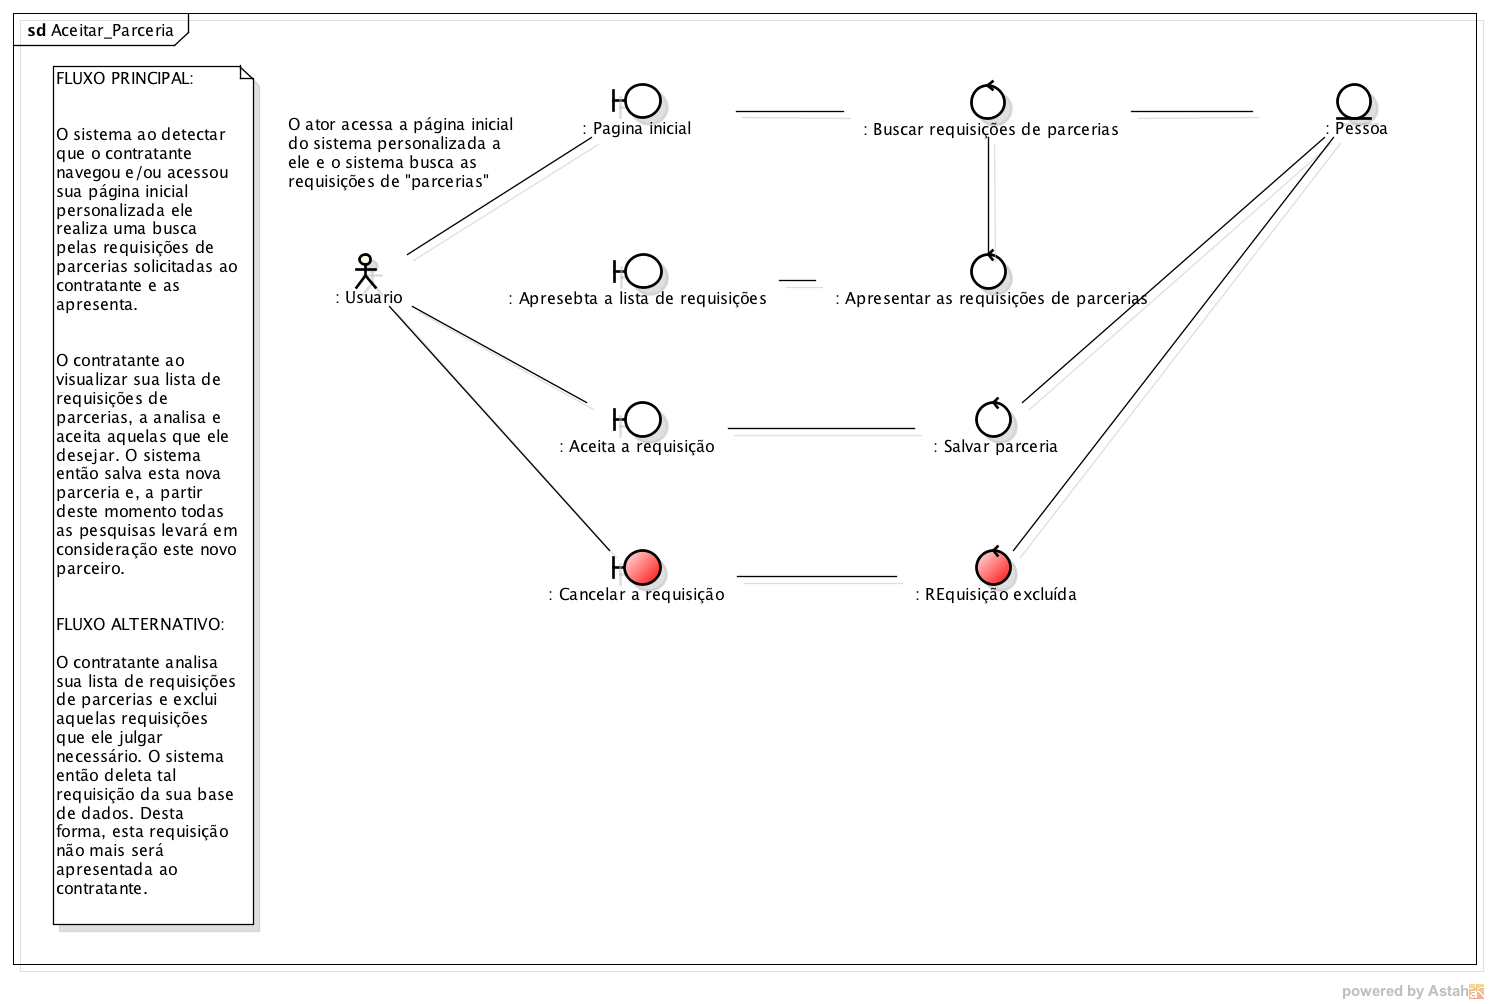
\includegraphics[scale=0.4]{./imagens/apendices/diagrama-robustez-aceitar-parceria.png}}
	\caption[Diagrama de robustez referente ao caso de uso ''Aceitar parceria''.]
	{Diagrama de robustez referente ao caso de uso ''Aceitar parceria''. \textbf{Fonte:} Elaborado pelos autores.}
	\label{fig:ap1:diagrama_robustez_aceitar_parceria}
\end{figure}

O próximo diagrama de robustez apresentado na Figura~\ref{fig:ap1:diagrama_robustez_localizar_parceiro} é referente ao caso de uso ''Localizar parceiro''.

\captionsetup[figure]{list=no}
\begin{figure}[h!]
	\centerline{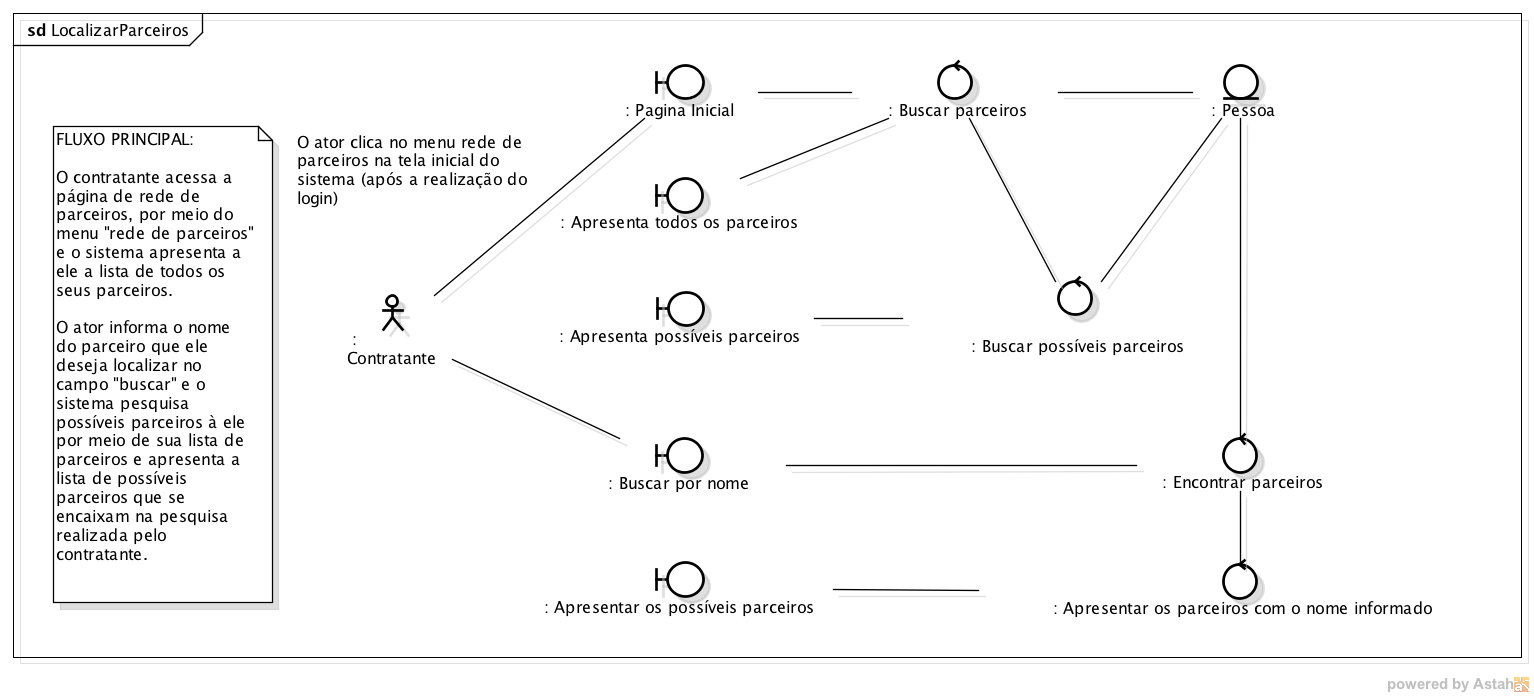
\includegraphics[scale=0.4]{./imagens/apendices/diagrama-robustez-localizar-parceiros.png}}
	\caption[Diagrama de robustez referente ao caso de uso ''Localizar parceiro''.]
	{Diagrama de robustez referente ao caso de uso ''Localizar parceiro''. \textbf{Fonte:} Elaborado pelos autores.}
	\label{fig:ap1:diagrama_robustez_localizar_parceiro}
\end{figure}

O próximo diagrama de robustez apresentado na Figura~\ref{fig:ap1:diagrama_robustez_adicionar_parceiro} é referente ao caso de uso ''Adicionar parceiro''.

\captionsetup[figure]{list=no}
\begin{figure}[h!]
	\centerline{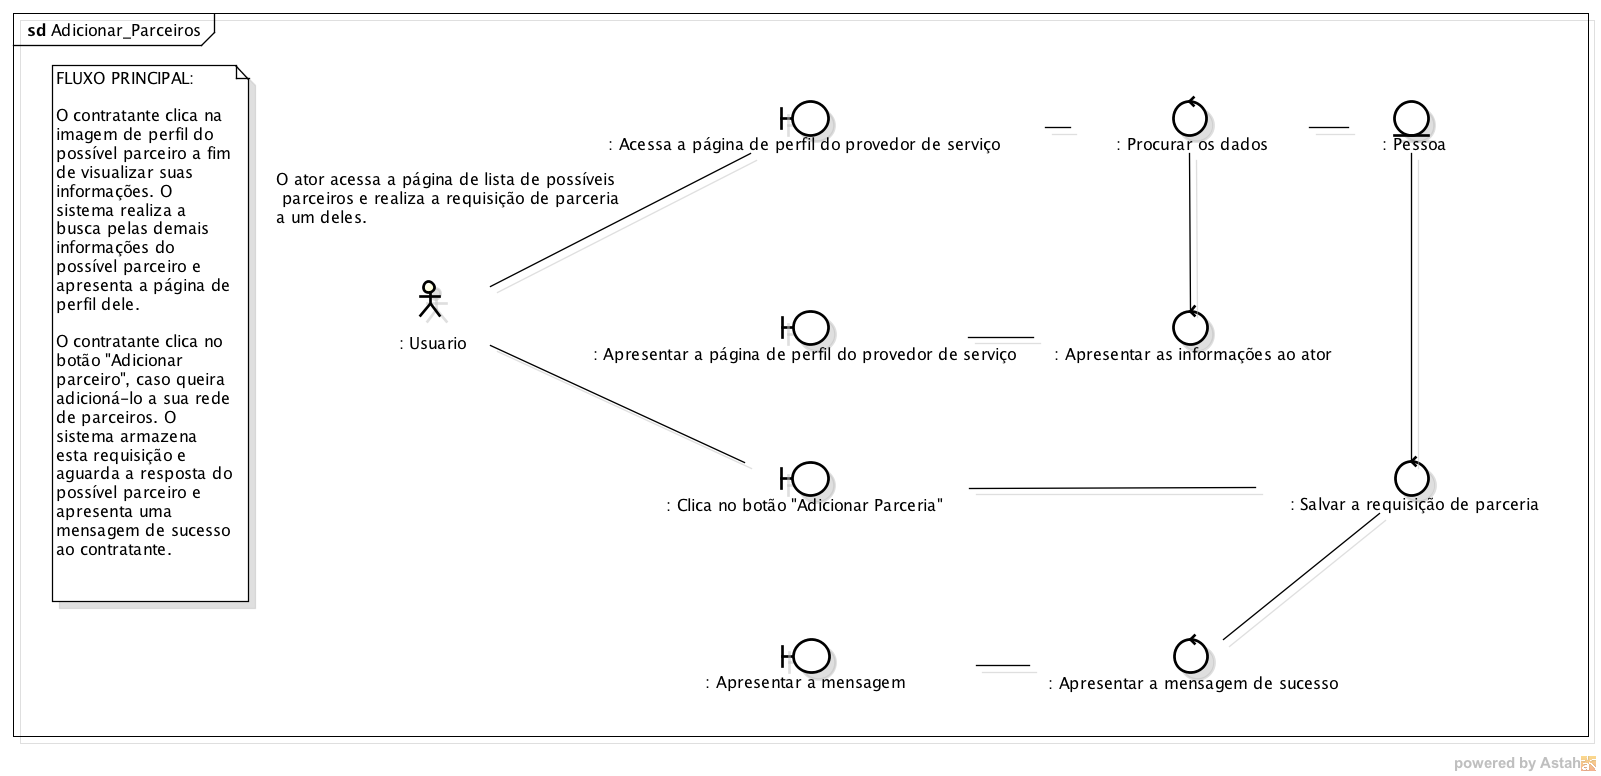
\includegraphics[scale=0.4]{./imagens/apendices/diagrama-robustez-adicionar-parceiro.png}}
	\caption[Diagrama de robustez referente ao caso de uso ''Adicionar parceiro''.]
	{Diagrama de robustez referente ao caso de uso ''Adicionar parceiro''. \textbf{Fonte:} Elaborado pelos autores.}
	\label{fig:ap1:diagrama_robustez_adicionar_parceiro}
\end{figure}

O próximo diagrama de robustez apresentado na Figura~\ref{fig:ap1:diagrama_robustez_localizar_mao_de_obra} é referente ao caso de uso ''Localizar mão de obra''.

\captionsetup[figure]{list=no}
\begin{figure}[h!]
	\centerline{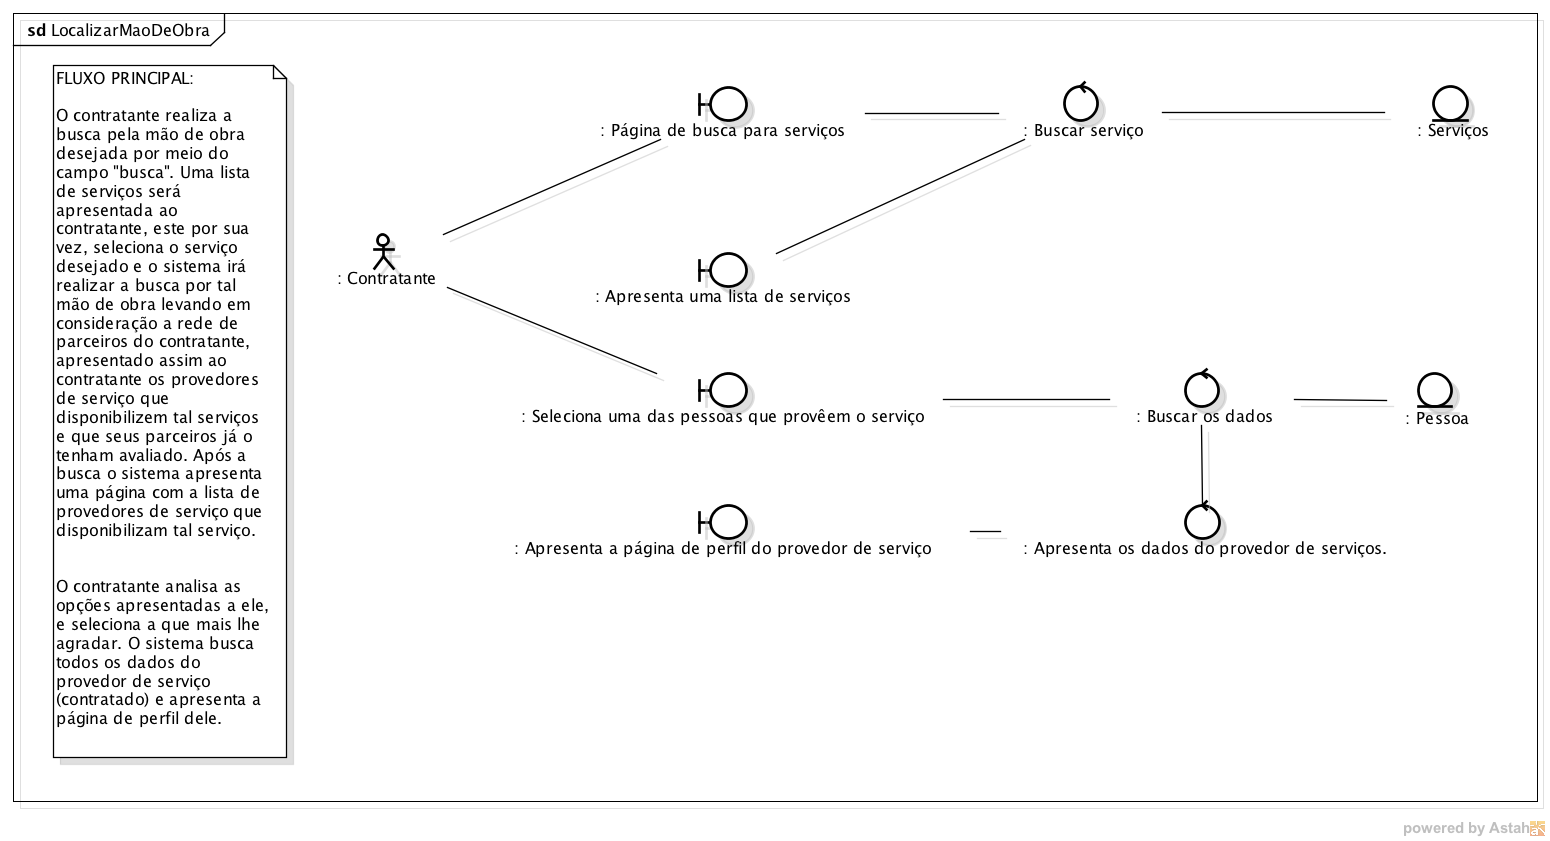
\includegraphics[scale=0.4]{./imagens/apendices/diagrama-robustez-localizar-mao-de-obra.png}}
	\caption[Diagrama de robustez referente ao caso de uso ''Localizar mão de obra''.]
	{Diagrama de robustez referente ao caso de uso ''Localizar mão de obra''. \textbf{Fonte:} Elaborado pelos autores.}
	\label{fig:ap1:diagrama_robustez_localizar_mao_de_obra}
\end{figure}

O próximo diagrama de robustez apresentado na Figura~\ref{fig:ap1:diagrama_robustez_avaliar_mao_de_obra} é referente ao caso de uso ''Avaliar mão de obra''.

\newpage
\captionsetup[figure]{list=no}
\begin{figure}[h!]
	\centerline{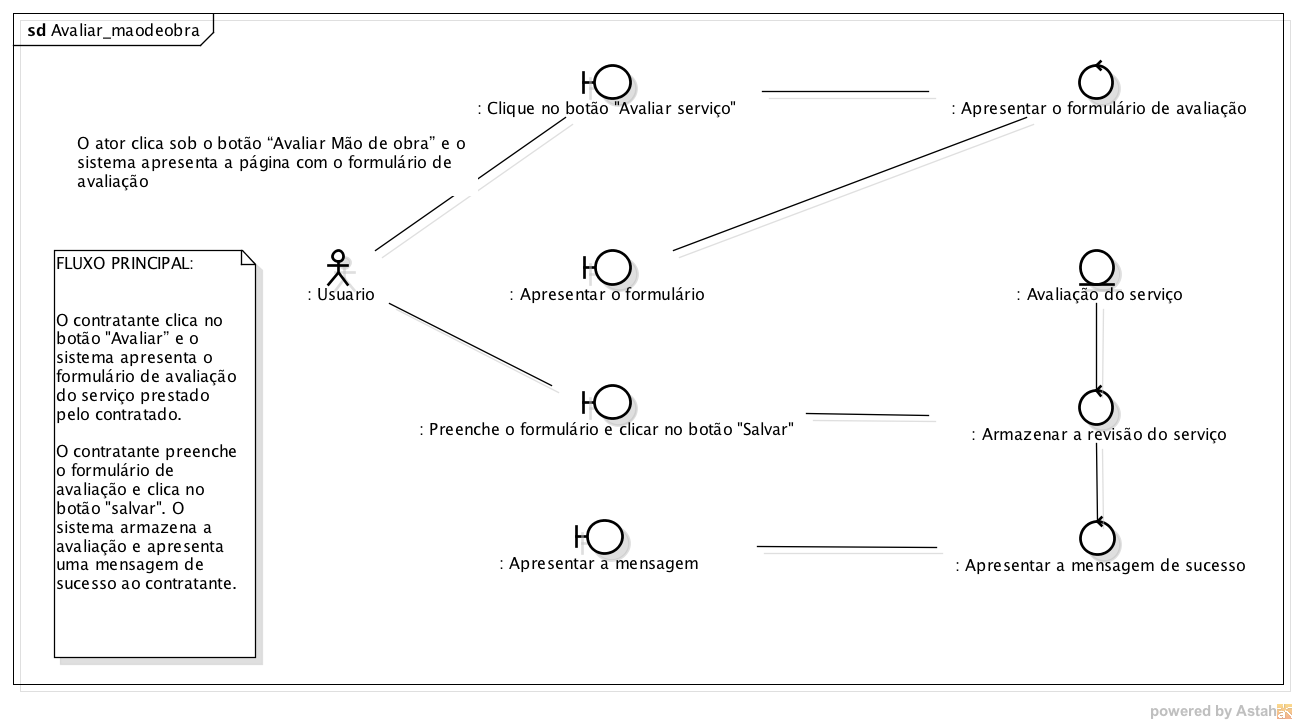
\includegraphics[scale=0.43]{./imagens/apendices/diagrama-robustez-avaliar-mao-de-obra.png}}
	\caption[Diagrama de robustez referente ao caso de uso ''Avaliar mão de obra''.]
	{Diagrama de robustez referente ao caso de uso ''Avaliar mão de obra''. \textbf{Fonte:} Elaborado pelos autores.}
	\label{fig:ap1:diagrama_robustez_avaliar_mao_de_obra}
\end{figure}

O próximo diagrama de robustez apresentado na Figura~\ref{fig:ap1:diagrama_robustez_gerenciar_servicos} é referente ao caso de uso ''Gerenciar serviços''.

\captionsetup[figure]{list=no}
\begin{figure}[h!]
	\centerline{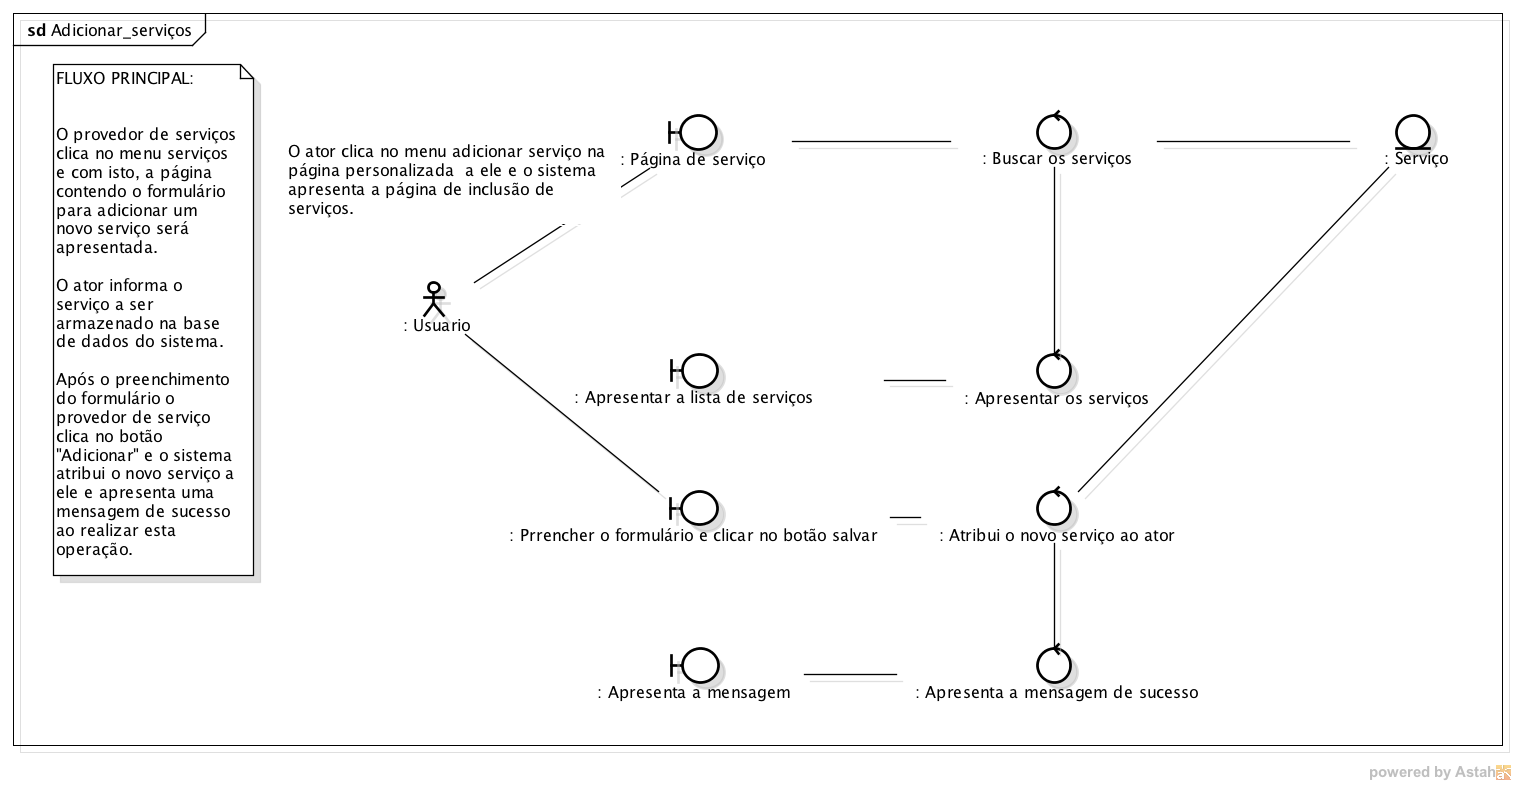
\includegraphics[scale=0.4]{./imagens/apendices/diagrama-robustez-adicionar-servicos.png}}
	\caption[Diagrama de robustez referente ao caso de uso ''Gerenciar serviços''.]
	{Diagrama de robustez referente ao caso de uso ''Gerenciar serviços''. \textbf{Fonte:} Elaborado pelos autores.}
	\label{fig:ap1:diagrama_robustez_gerenciar_servicos}
\end{figure}

O último diagrama de robustez apresentado na Figura~\ref{fig:ap1:diagrama_robustez_criar_conta} é referente ao caso de uso ''Criar conta''.

\newpage
\captionsetup[figure]{list=no}
\begin{figure}[h!]
	\centerline{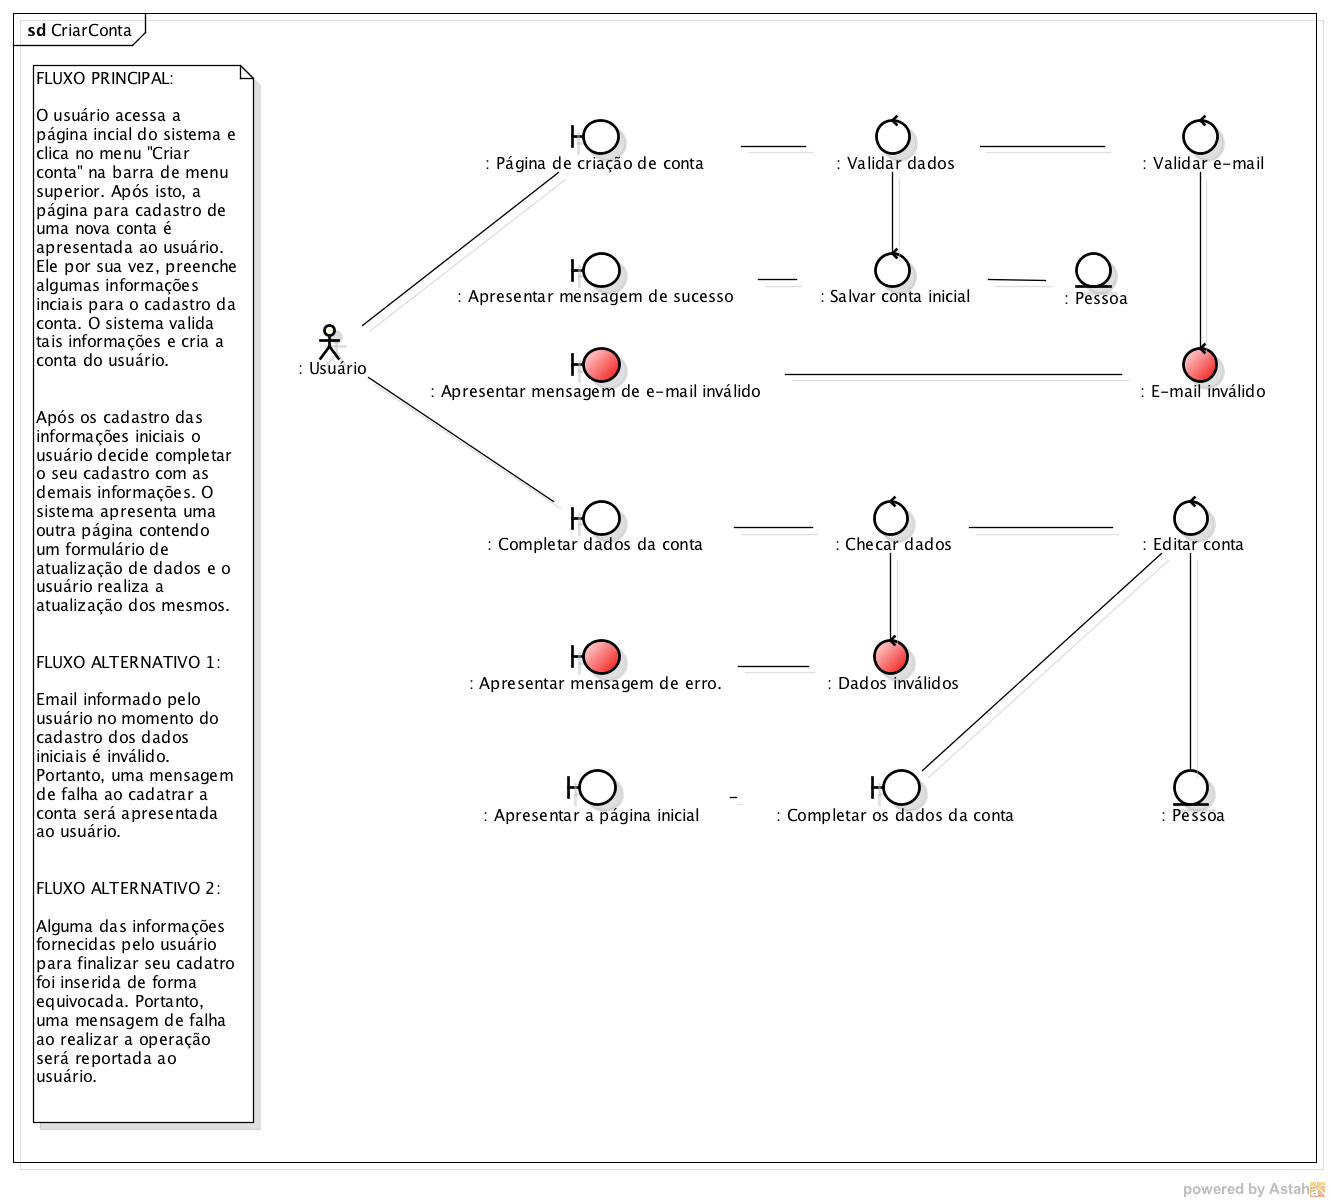
\includegraphics[scale=0.4]{./imagens/apendices/diagrama-robustez-criar-conta.png}}
	\caption[Diagrama de robustez referente ao caso de uso ''Criar conta''.]
	{Diagrama de robustez referente ao caso de uso ''Criar conta''. \textbf{Fonte:} Elaborado pelos autores.}
	\label{fig:ap1:diagrama_robustez_criar_conta}
\end{figure}

Após a criação dos diagramas de robustez, o diagrama de modelo de domínio foi atualizado, adicionando os atributos identificados pelos diagramas de caso de robustez, passando-se a trabalhar nos diagramas de sequência, que seão apresentados a seguir.

\section*{Diagramas de Sequência}

Os diagramas de sequência foram criados baseado-se no diagramas apresentados anteriormente. Seguindo a mesma ordem anteriormente definida, o primeiro diagrama de sequência apresentado na Figura~\ref{fig:ap1:diagrama_sequencia_aceitar_parceria} é referente ao caso de uso ''Aceitar parceria''.

\newpage
\captionsetup[figure]{list=no}
\begin{figure}[h!]
	\centerline{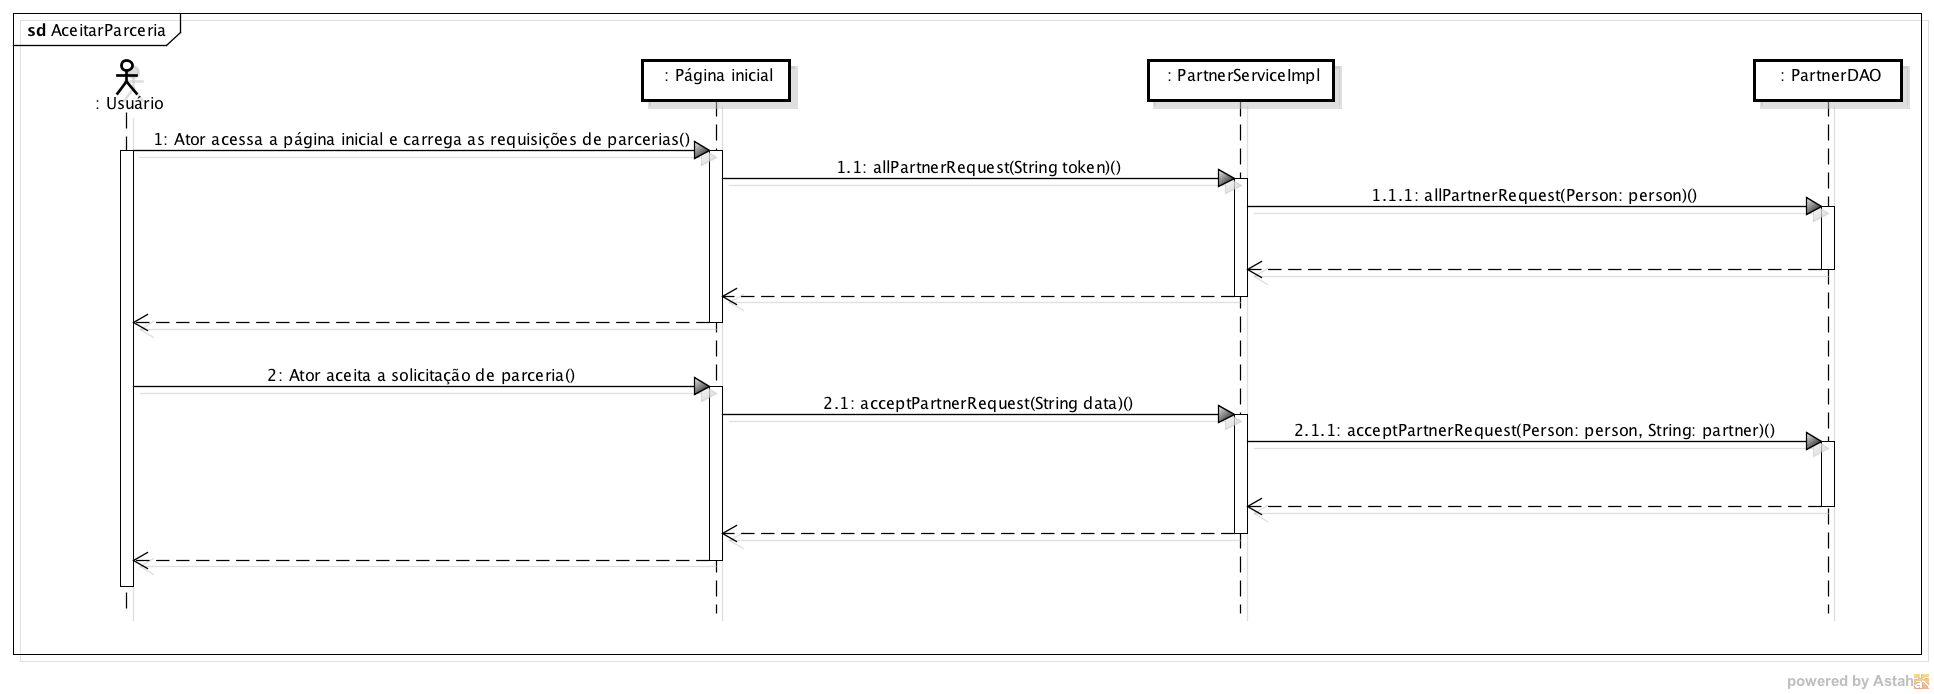
\includegraphics[angle=90,scale=0.45]{./imagens/apendices/diagrama-sequencia-aceitar-parceria.png}}
	\caption[Diagrama de sequência referente ao caso de uso ''Aceitar parceria''.]
	{Diagrama de robustez sequência ao caso de uso ''Aceitar parceria''. \textbf{Fonte:} Elaborado pelos autores.}
	\label{fig:ap1:diagrama_sequencia_aceitar_parceria}
\end{figure}


O próximo diagrama de sequência apresentado na Figura~\ref{fig:ap1:diagrama_sequencia_localizar_parceiro} é referente ao caso de uso ''Localizar parceiro''.

\captionsetup[figure]{list=no}
\begin{figure}[h!]
	\centerline{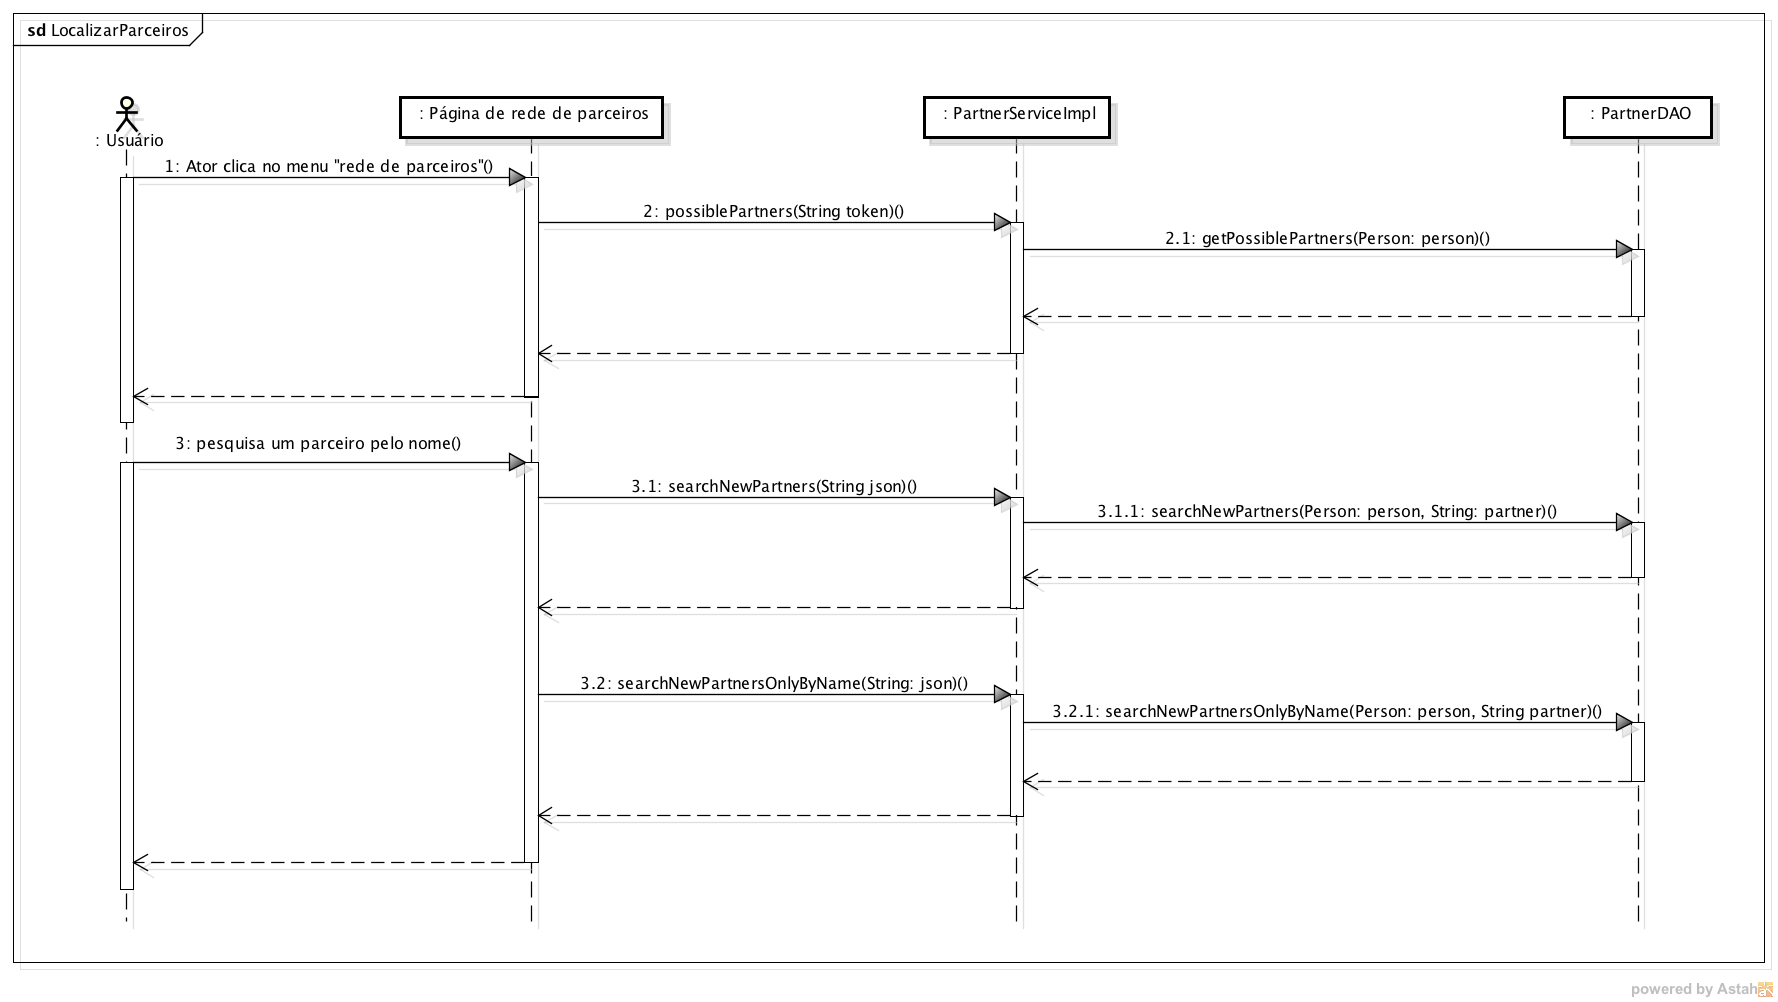
\includegraphics[angle=90,scale=0.45]{./imagens/apendices/diagrama-sequencia-localizar-parceiros.png}}
	\caption[Diagrama de sequência referente ao caso de uso ''Localizar parceiro''.]
	{Diagrama de sequência referente ao caso de uso ''Localizar parceiro''. \textbf{Fonte:} Elaborado pelos autores.}
	\label{fig:ap1:diagrama_sequencia_localizar_parceiro}
\end{figure}

O próximo diagrama de sequência apresentado na Figura~\ref{fig:ap1:diagrama_sequencia_adicionar_parceiro} é referente ao caso de uso ''Adicionar parceiro''.

\captionsetup[figure]{list=no}
\begin{figure}[h!]
	\centerline{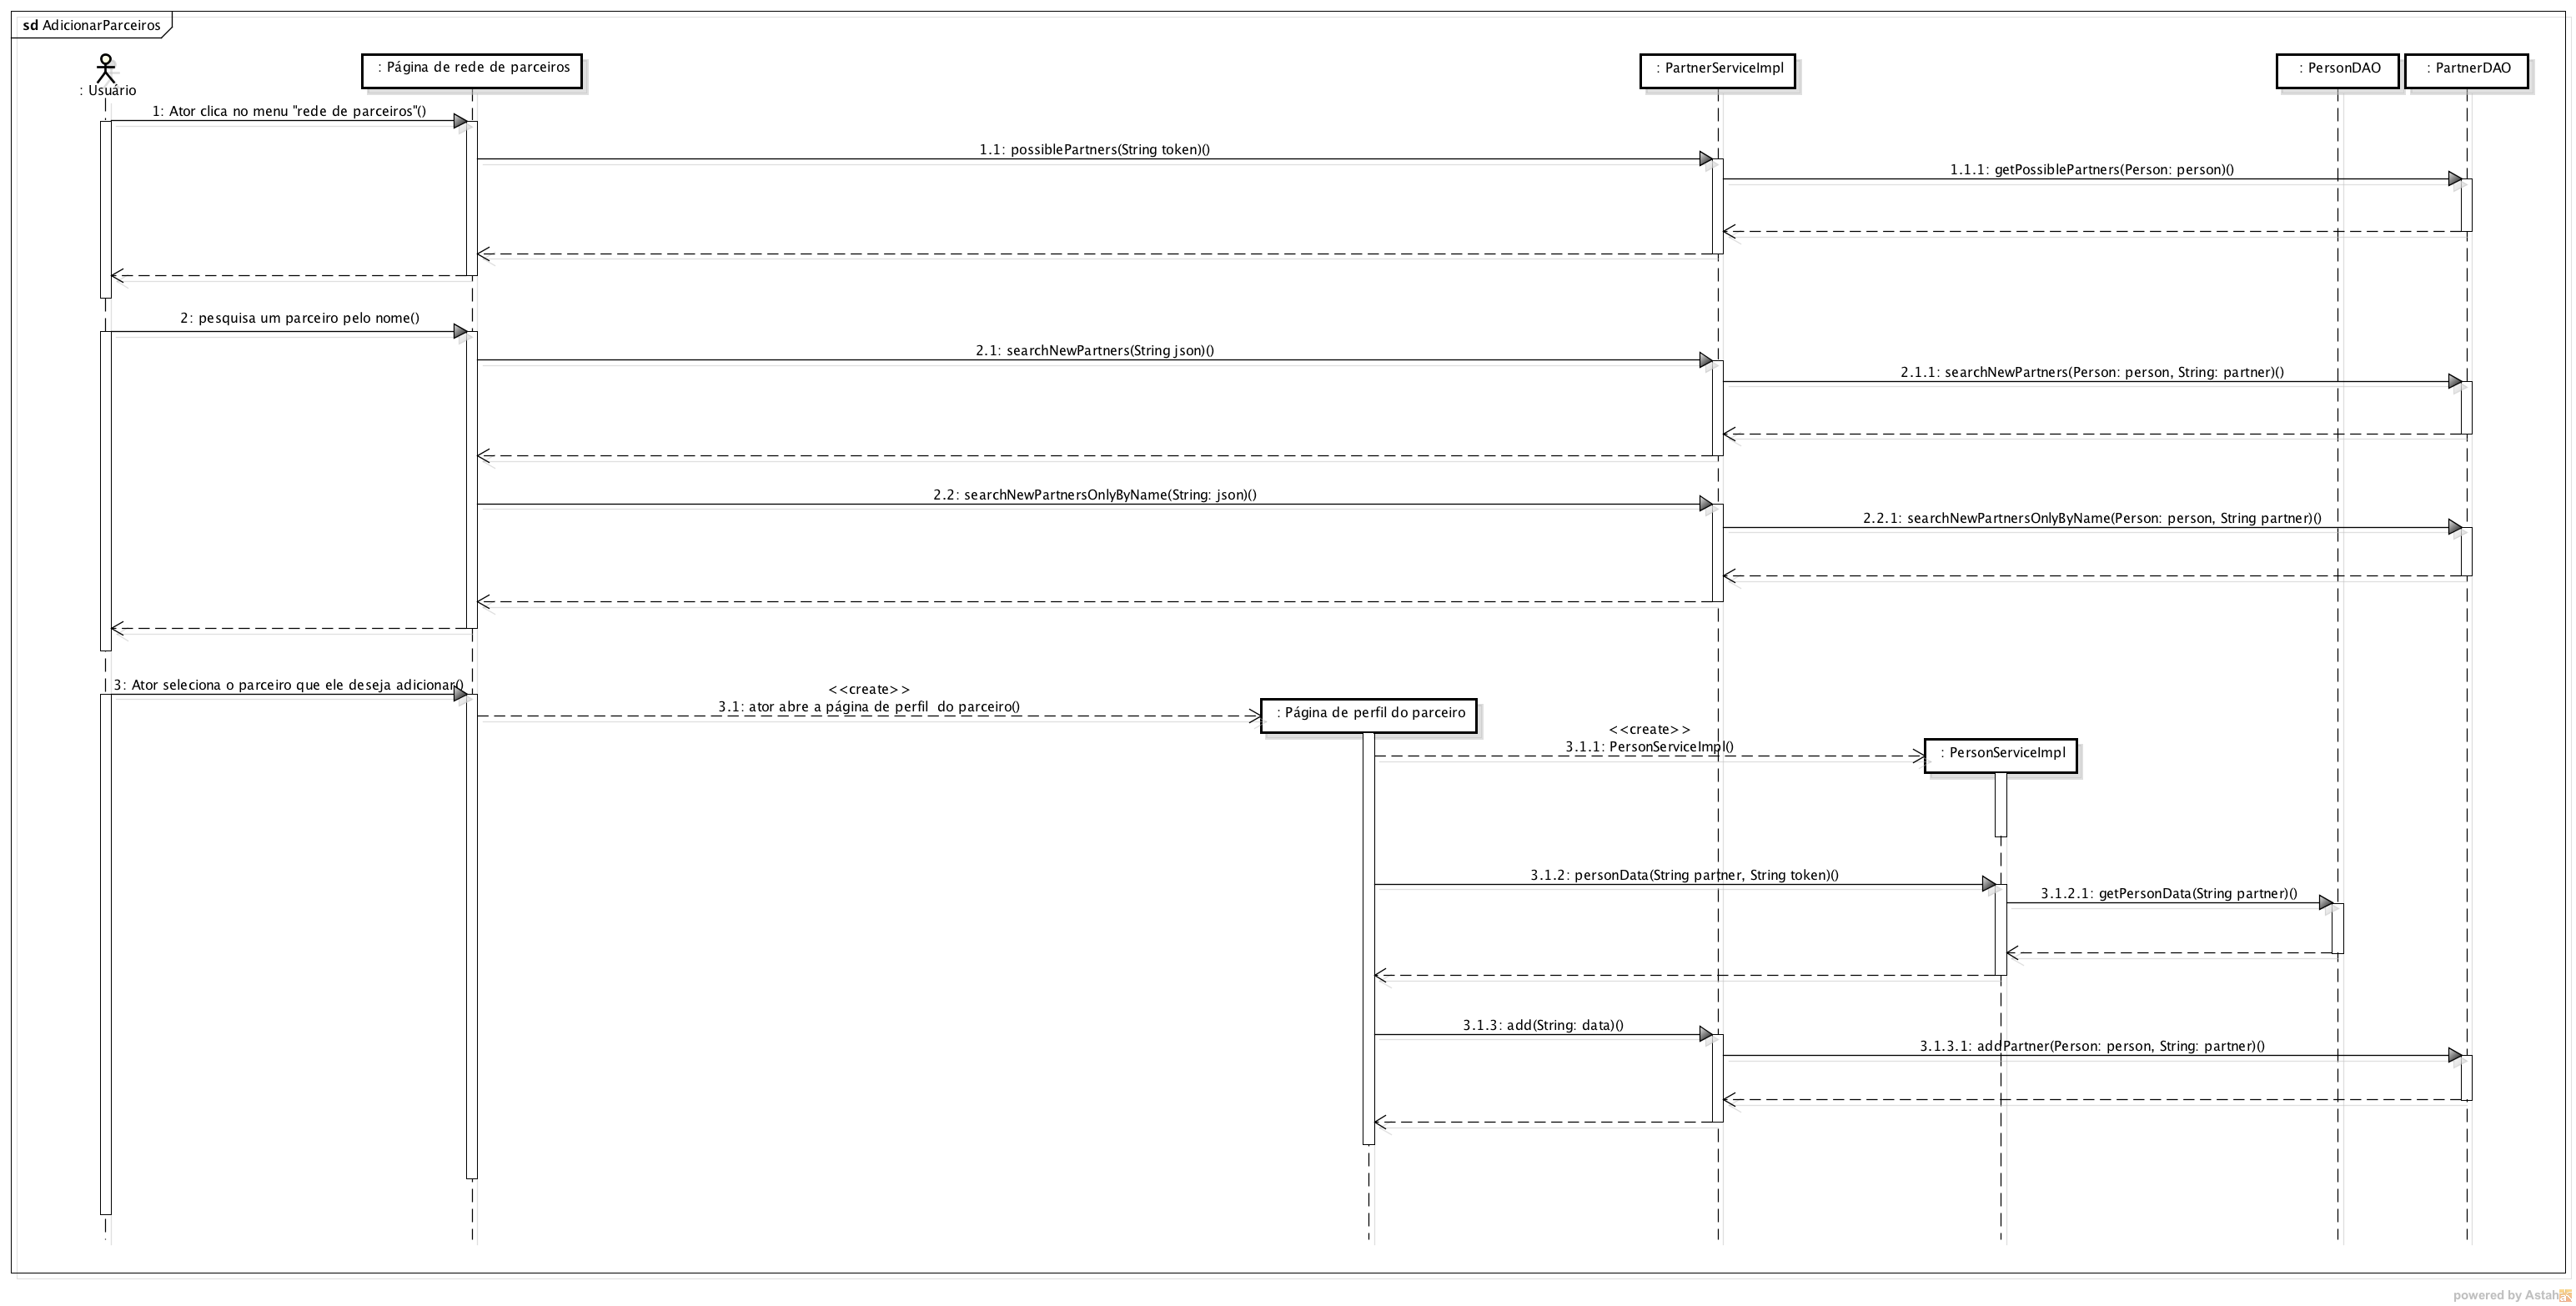
\includegraphics[angle=90,scale=0.25]{./imagens/apendices/diagrama-sequencia-adicionar-parceiros.png}}
	\caption[Diagrama de sequência referente ao caso de uso ''Adicionar parceiro''.]
	{Diagrama de sequência referente ao caso de uso ''Adicionar parceiro''. \textbf{Fonte:} Elaborado pelos autores.}
	\label{fig:ap1:diagrama_sequencia_adicionar_parceiro}
\end{figure}

O próximo diagrama de sequência apresentado na Figura~\ref{fig:ap1:diagrama_sequencia_localizar_mao_de_obra} é referente ao caso de uso ''Localizar mão de obra''.

\captionsetup[figure]{list=no}
\begin{figure}[h!]
	\centerline{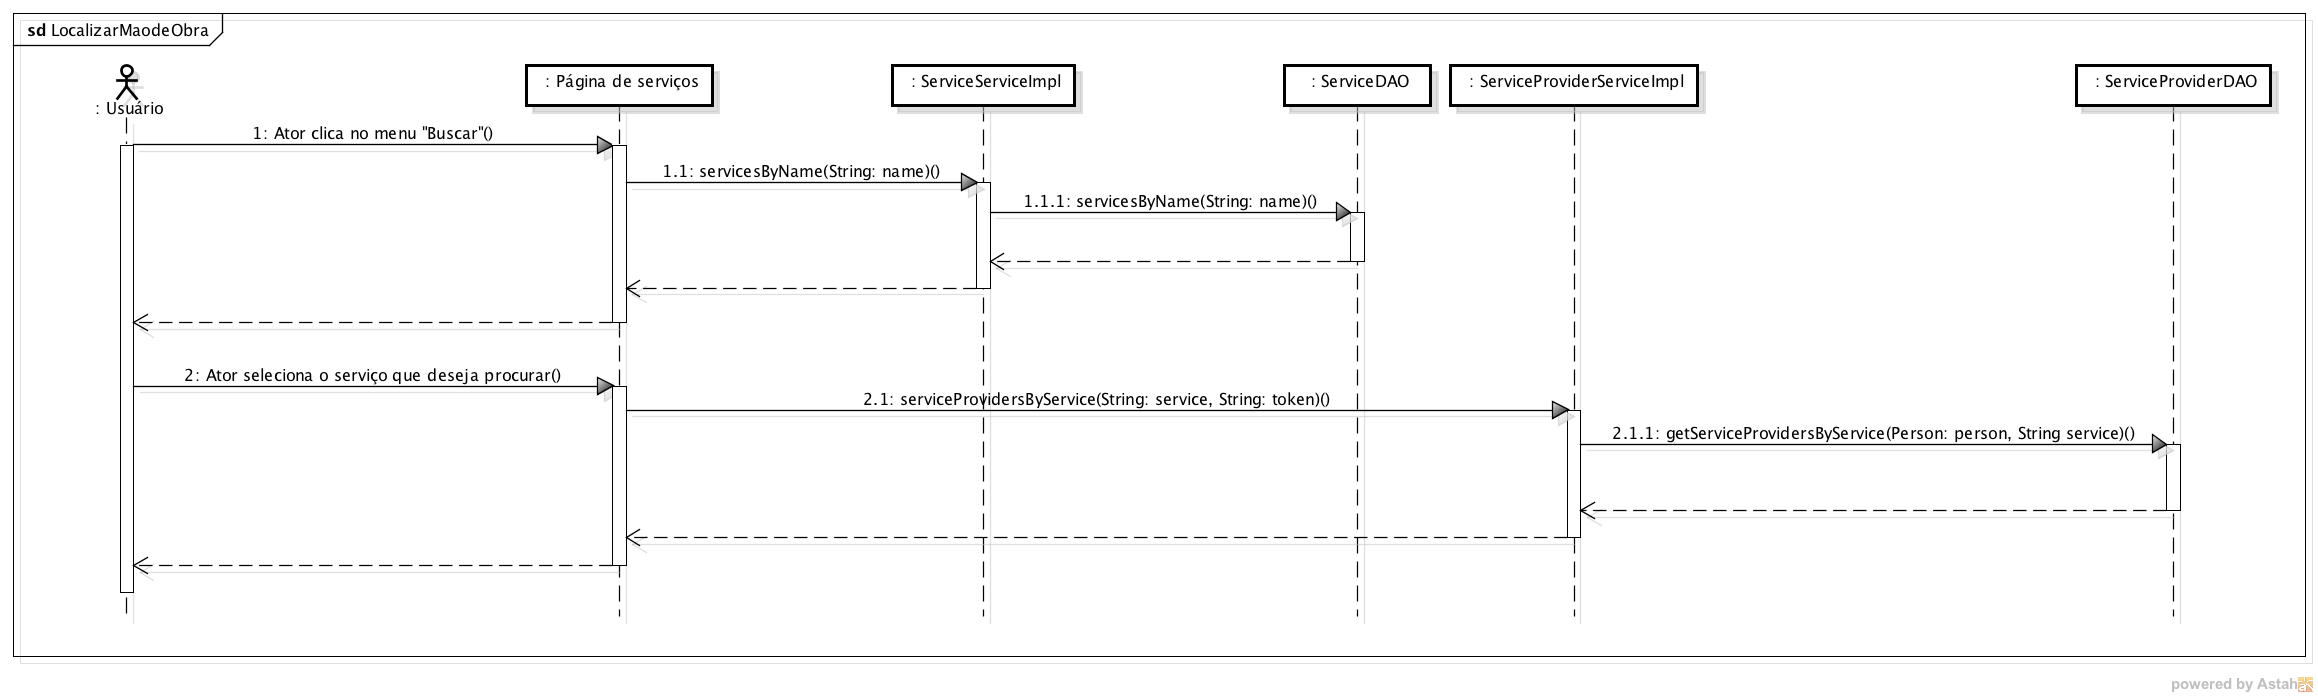
\includegraphics[angle=90,scale=0.35]{./imagens/apendices/diagrama-sequencia-localizar-mao-de-obra.png}}
	\caption[Diagrama de sequência referente ao caso de uso ''Localizar mão de obra''.]
	{Diagrama de robustez sequência ao caso de uso ''Localizar mão de obra''. \textbf{Fonte:} Elaborado pelos autores.}
	\label{fig:ap1:diagrama_sequencia_localizar_mao_de_obra}
\end{figure}

O próximo diagrama de sequência apresentado na Figura~\ref{fig:ap1:diagrama_sequencia_avaliar_mao_de_obra} é referente ao caso de uso ''Avaliar mão de obra''.

\captionsetup[figure]{list=no}
\begin{figure}[h!]
	\centerline{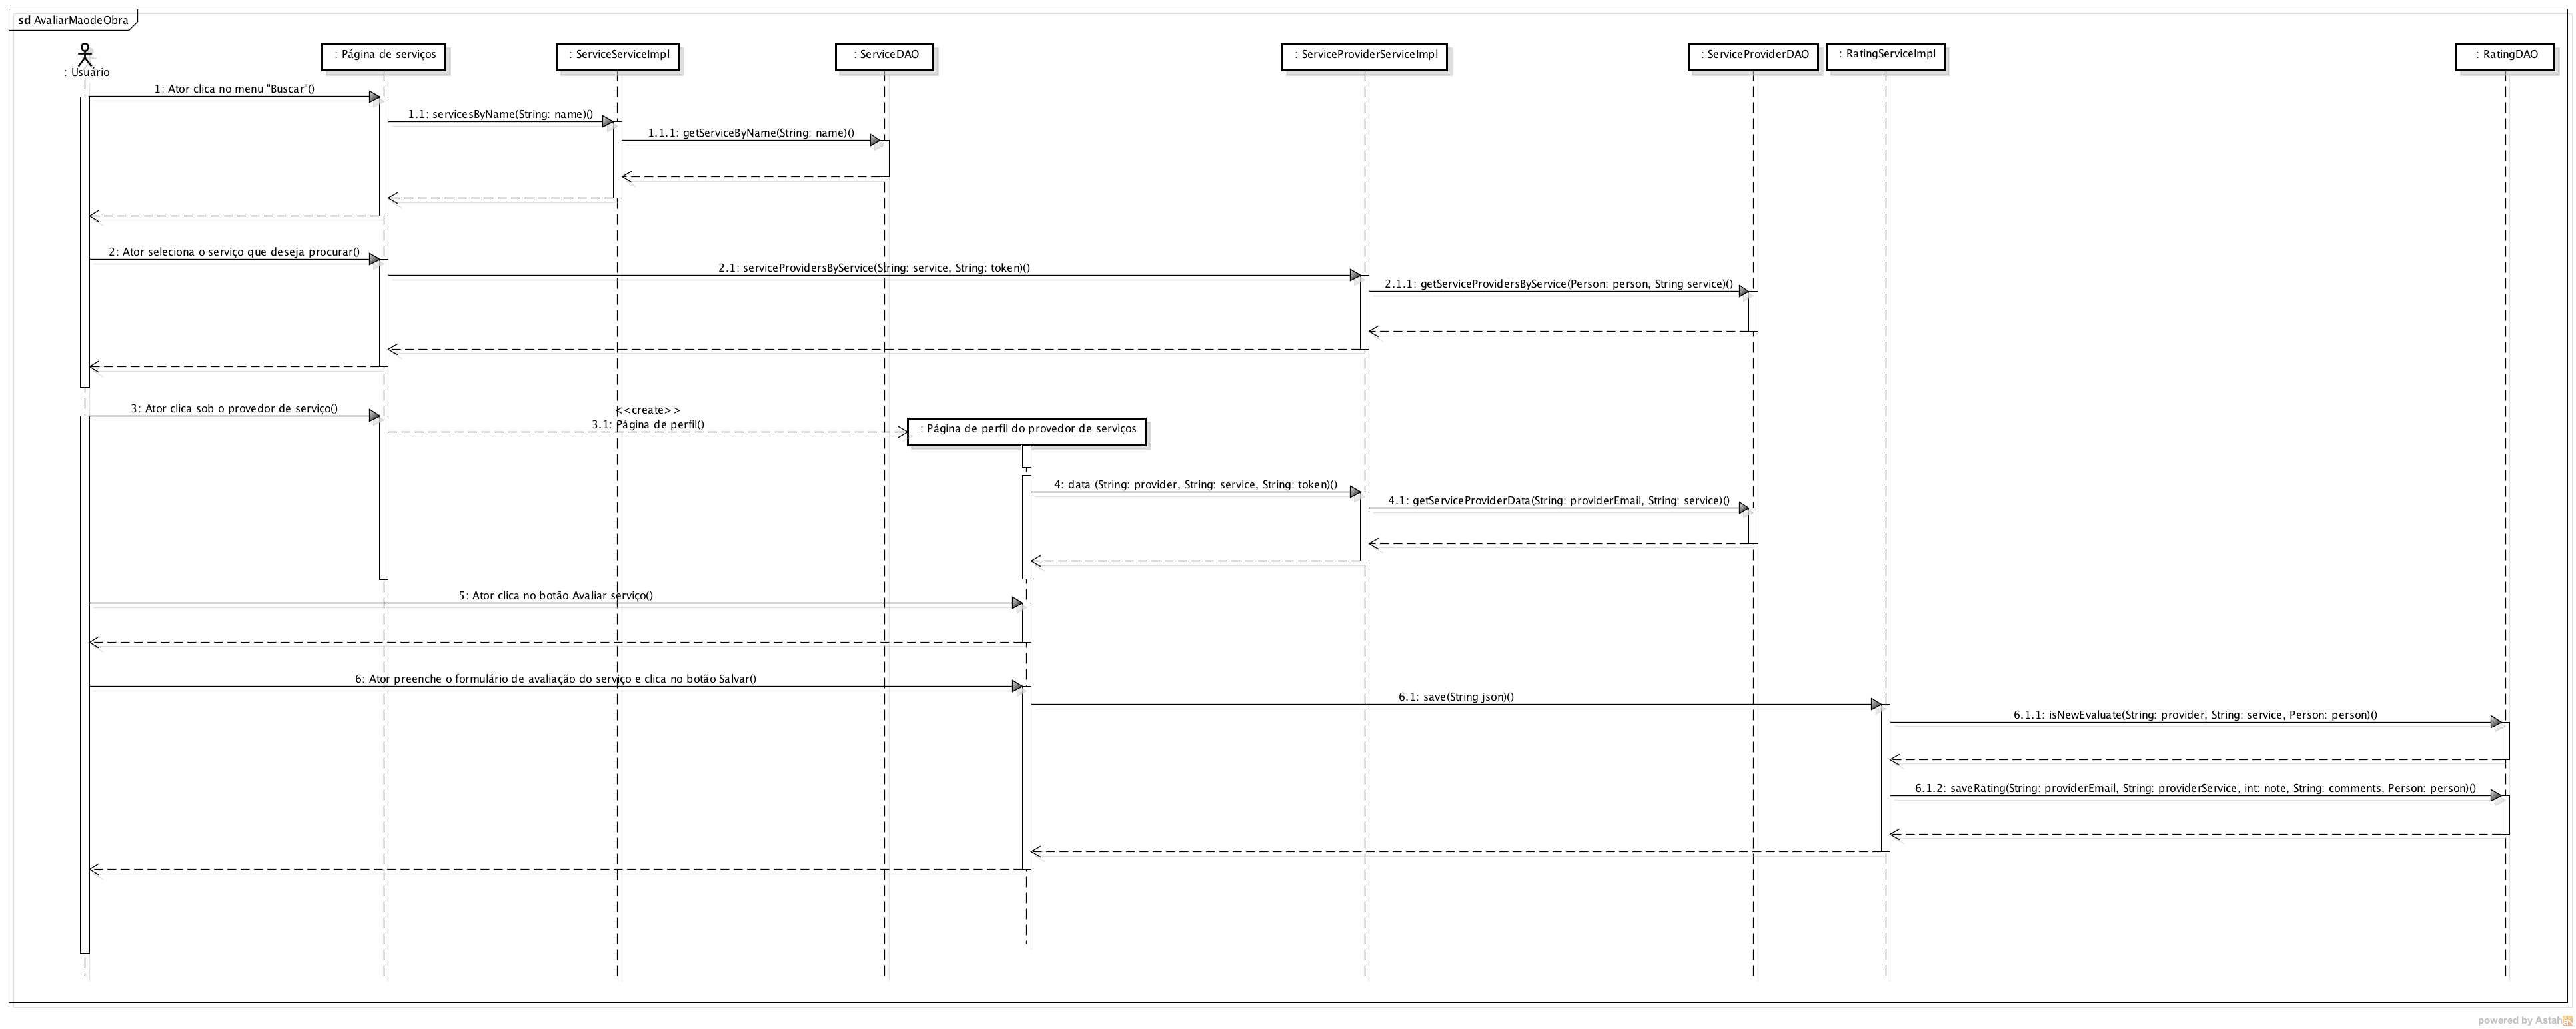
\includegraphics[angle=90,scale=0.17]{./imagens/apendices/diagrama-sequencia-avaliar-mao-de-obra.png}}
	\caption[Diagrama de sequência referente ao caso de uso ''Avaliar mão de obra''.]
	{Diagrama de robustez sequência ao caso de uso ''Avaliar mão de obra''. \textbf{Fonte:} Elaborado pelos autores.}
	\label{fig:ap1:diagrama_sequencia_avaliar_mao_de_obra}
\end{figure}

O próximo diagrama de sequência apresentado na Figura~\ref{fig:ap1:diagrama_sequencia_gerenciar_servicos} é referente ao caso de uso ''Gerenciar serviços''.

\newpage
\captionsetup[figure]{list=no}
\begin{figure}[h!]
	\centerline{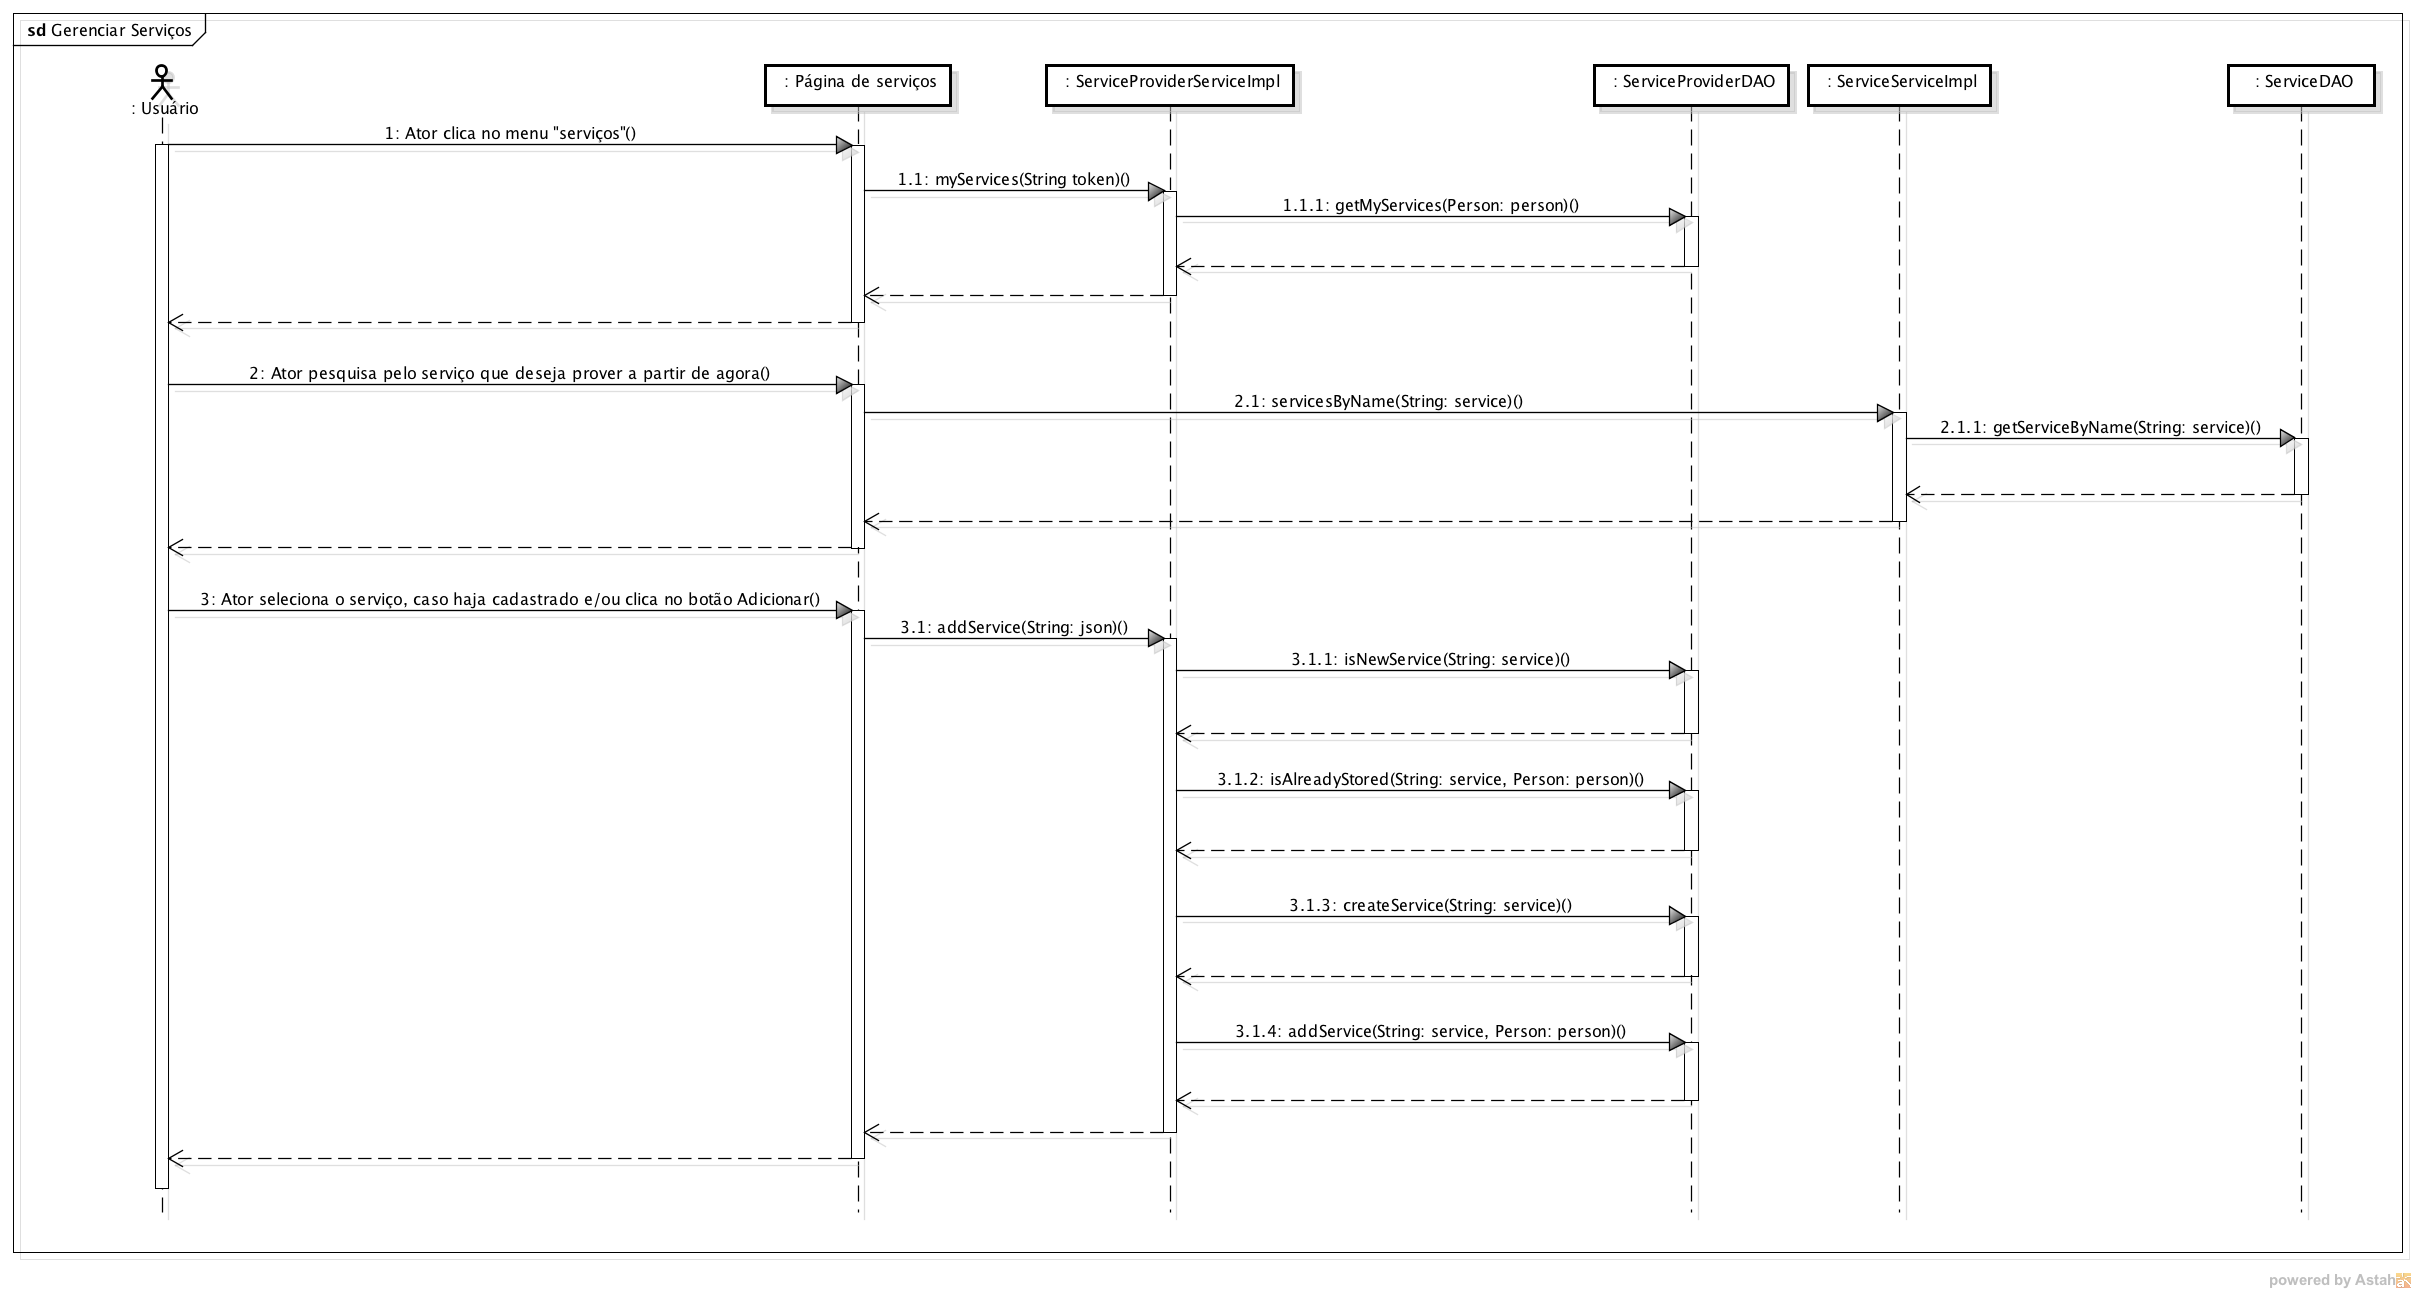
\includegraphics[angle=90,scale=0.35]{./imagens/apendices/diagrama-sequencia-gerenciar-servicos.png}}
	\caption[Diagrama de sequência referente ao caso de uso ''Gerenciar serviços''.]
	{Diagrama de sequência referente ao caso de uso ''Gerenciar serviços''. \textbf{Fonte:} Elaborado pelos autores.}
	\label{fig:ap1:diagrama_sequencia_gerenciar_servicos}
\end{figure}

O último diagrama de sequência apresentado na Figura~\ref{fig:ap1:diagrama_sequencia_criar_conta} é referente ao caso de uso ''Criar conta''.

\captionsetup[figure]{list=no}
\begin{figure}[h!]
	\centerline{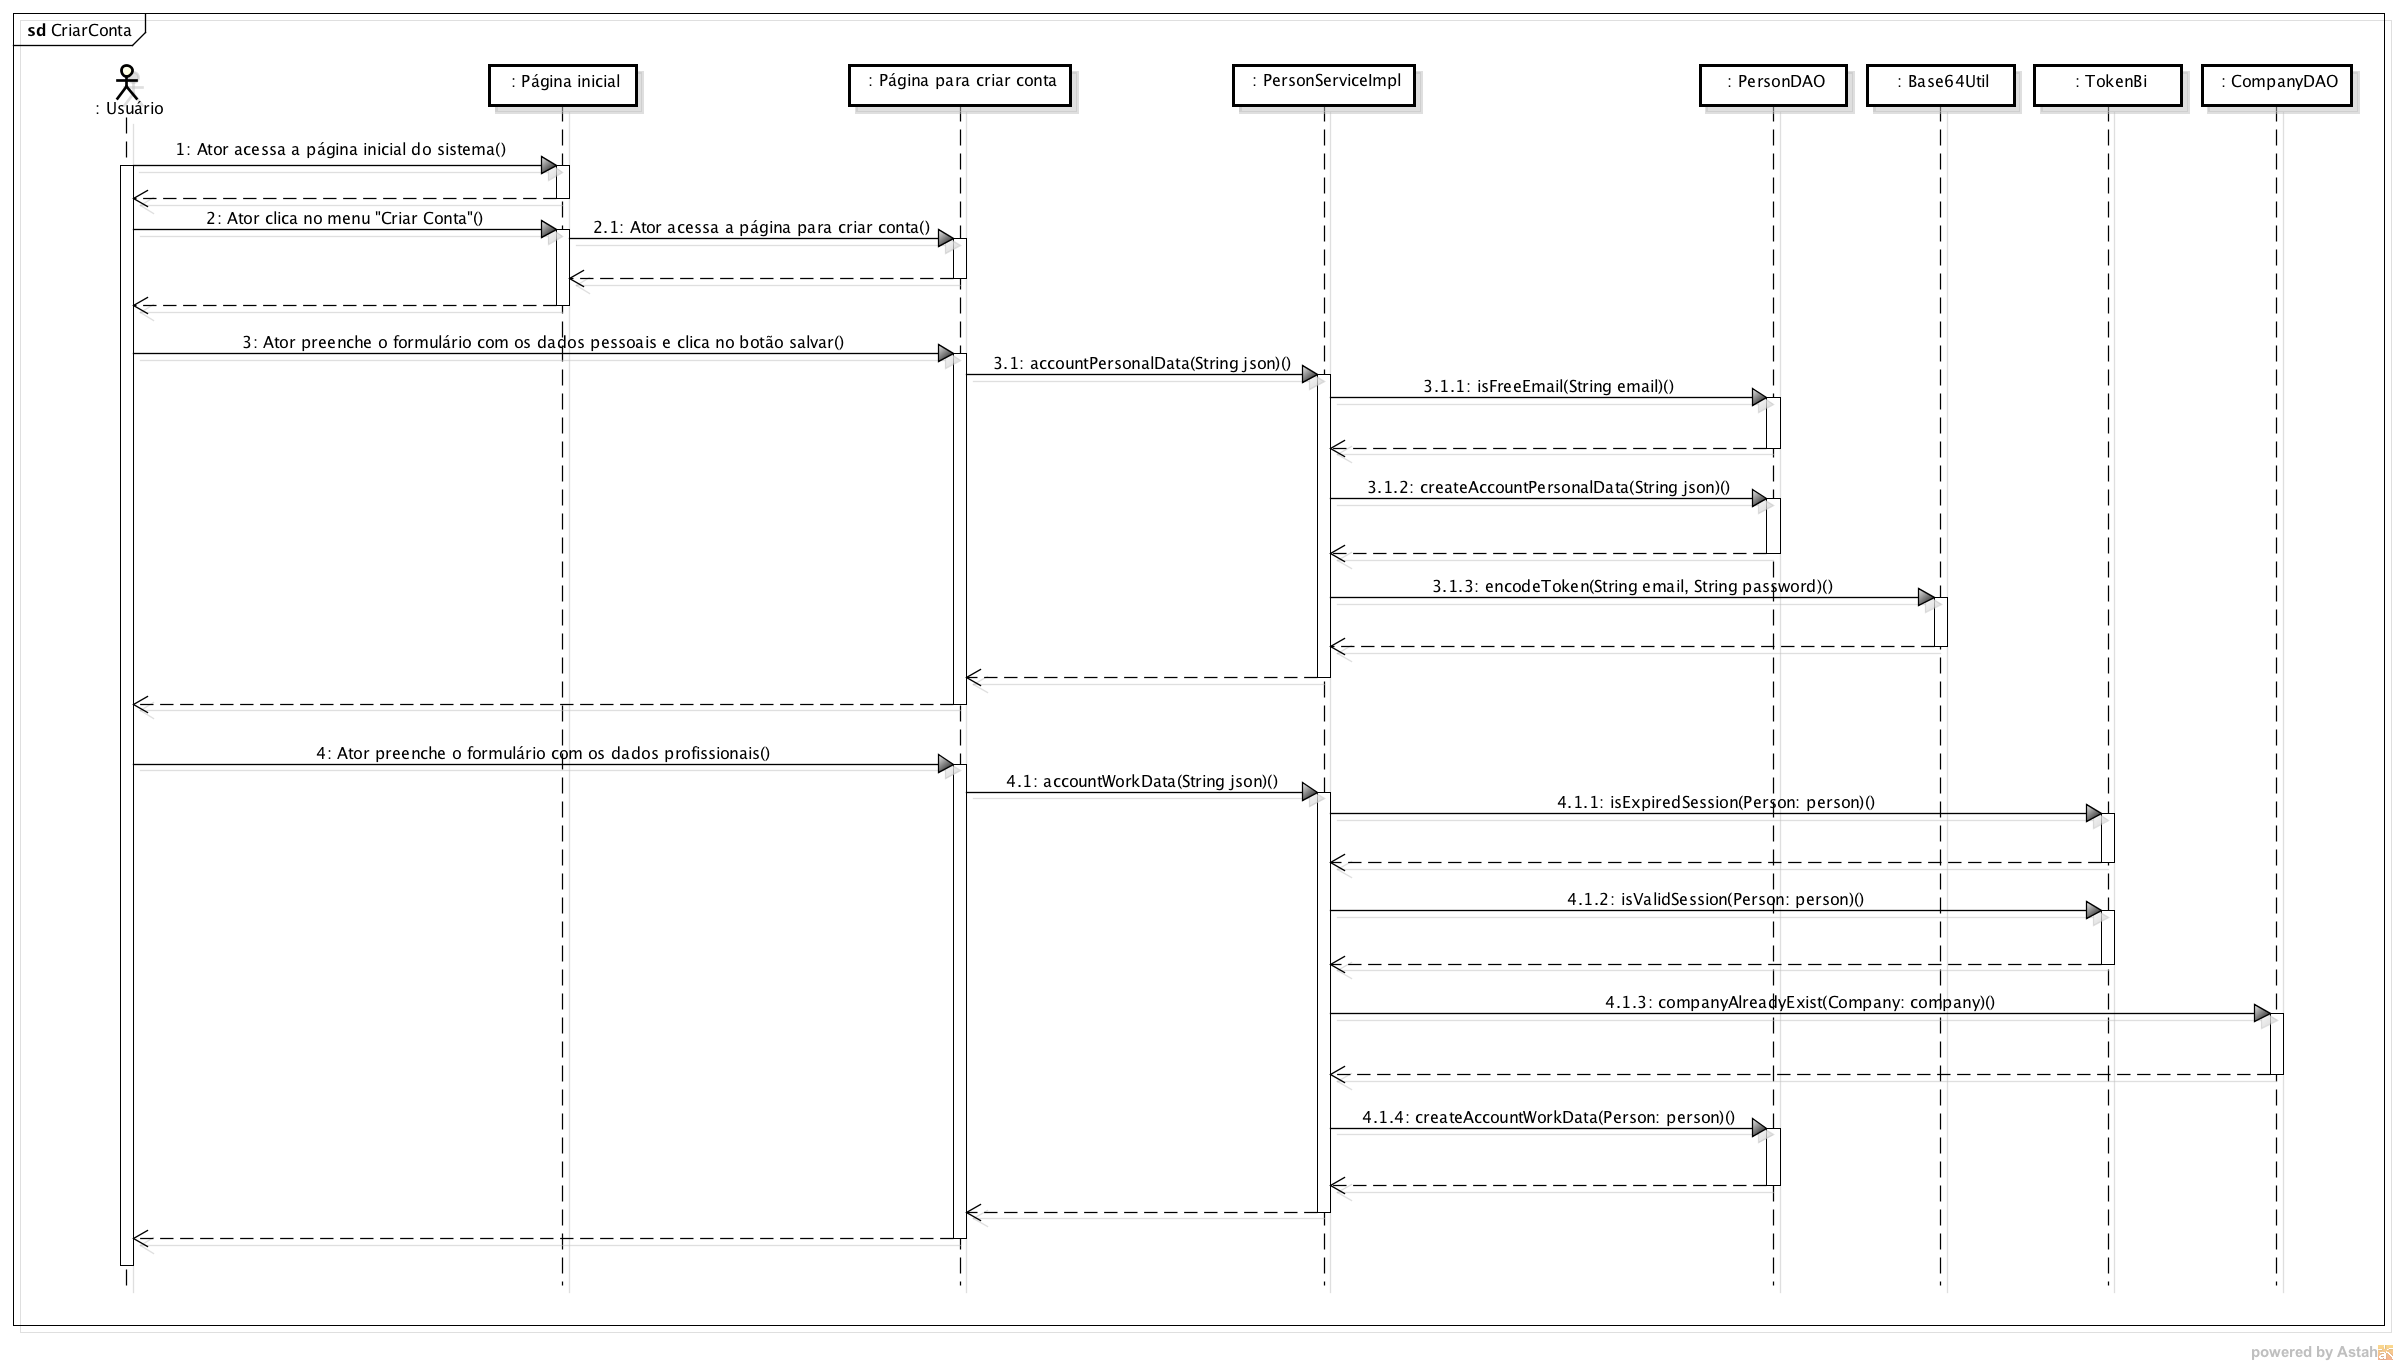
\includegraphics[angle=90,scale=0.35]{./imagens/apendices/diagrama-sequencia-criar-conta.png}}
	\caption[Diagrama de sequência referente ao caso de uso ''Criar conta''.]
	{Diagrama de sequência referente ao caso de uso ''Criar conta''. \textbf{Fonte:} Elaborado pelos autores.}
	\label{fig:ap1:diagrama_sequencia_criar_conta}
\end{figure}


Após a criação dos diagramas de sequência, o diagrama de modelo de domínio foi atualizado, adicionando os atributos identificados pelos diagramas de sequência, gerando o diagrama de classes final.
